\documentclass[tikz,border=8pt]{standalone}
\usepackage{amsmath}
\usetikzlibrary{arrows.meta,decorations.pathmorphing,calc}
\definecolor{ink}{HTML}{21352F}
\definecolor{teal}{HTML}{087F7B}
\definecolor{gold}{HTML}{C58B2A}
\definecolor{blue}{HTML}{4B77A8}
\definecolor{rose}{HTML}{B65A62}
\begin{document}
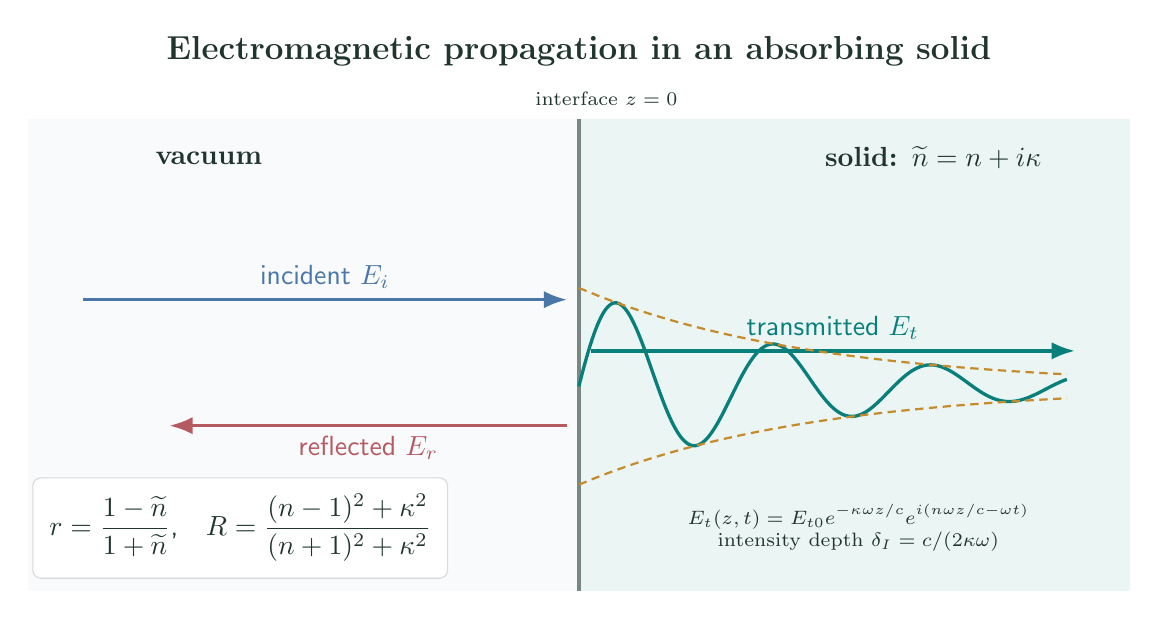
\begin{tikzpicture}[font=\sffamily,text=ink,>=Latex]
  \node[font=\bfseries\large] at (0,4.05) {Electromagnetic propagation in an absorbing solid};
  \fill[blue!4] (-7,-2.8) rectangle (0,3.2);
  \fill[teal!8] (0,-2.8) rectangle (7,3.2);
  \draw[ink!60,very thick] (0,-2.8)--(0,3.2);
  \node[font=\bfseries] at (-4.7,2.7) {vacuum};
  \node[font=\bfseries] at (4.5,2.7) {solid: $\widetilde n=n+i\kappa$};
  \draw[->,blue,very thick] (-6.3,.9)--(-.15,.9) node[midway,above] {incident $E_i$};
  \draw[->,rose,very thick] (-.15,-.7)--(-5.2,-.7) node[midway,below] {reflected $E_r$};
  \draw[->,teal,very thick] (.15,.25)--(6.3,.25) node[midway,above] {transmitted $E_t$};
  \draw[teal,very thick,smooth,domain=0:6.2,samples=180,variable=\x]
    plot ({\x},{-.2+1.25*exp(-.34*\x)*sin(180*\x)});
  \draw[gold,densely dashed,thick,smooth,domain=0:6.2,samples=80,variable=\x]
    plot ({\x},{-.2+1.25*exp(-.34*\x)});
  \draw[gold,densely dashed,thick,smooth,domain=0:6.2,samples=80,variable=\x]
    plot ({\x},{-.2-1.25*exp(-.34*\x)});
  \node[font=\scriptsize,align=center] at (3.55,-2.0)
    {$\displaystyle E_t(z,t)=E_{t0}e^{-\kappa\omega z/c}e^{i(n\omega z/c-\omega t)}$\\
     intensity depth $\delta_I=c/(2\kappa\omega)$};
  \node[draw=ink!18,rounded corners=3pt,fill=white,inner sep=6pt,align=center] at (-4.3,-2.0)
    {$\displaystyle r=\frac{1-\widetilde n}{1+\widetilde n}$,\quad
     $\displaystyle R=\frac{(n-1)^2+\kappa^2}{(n+1)^2+\kappa^2}$};
  \node[font=\scriptsize] at (.35,3.45) {interface $z=0$};
\end{tikzpicture}
\end{document}
